\documentclass[11pt]{article}
\usepackage{graphicx} % Required for inserting images
\usepackage{hyperref}
\usepackage{listings}
\usepackage{caption}
\usepackage{minted}
\usepackage{todonotes}
\usepackage[a4paper, total={6in, 8in},margin=1in,top=0.81in,bottom=1.25in]{geometry}
\usepackage{fancyhdr}
\usepackage{pdfpages}
\usepackage{sectsty}
\usepackage{fontspec}

\setmainfont{Carlito}
\sectionfont{\fontsize{24}{30}\selectfont}  % 24pt size, 30pt line spacing
\subsectionfont{\fontsize{18}{24}\selectfont}
\subsubsectionfont{\fontsize{14}{18}\selectfont}
\renewcommand{\listingscaption}{Izvorni kod}
\renewcommand{\listoflistingscaption}{Spisak izvornih kodova}
\pagestyle{fancy}
\fancyhf{}
\fancyfoot[L]{\fontsize{11}{13}\selectfont Aleksa Bajat, Intermedijarne reprezentacije izvornog koda u prednjem kraju (frontend-u) rustc kompajlera}
\fancyfoot[R]{\newline\fontsize{11}{13}\selectfont \thepage}

\title{Intermedijarne reprezentacije izvornog koda u prednjem kraju (frontend-u) rustc kompajlera}
\author{Aleksa Bajat}
\date{September 2024}

\begin{document}
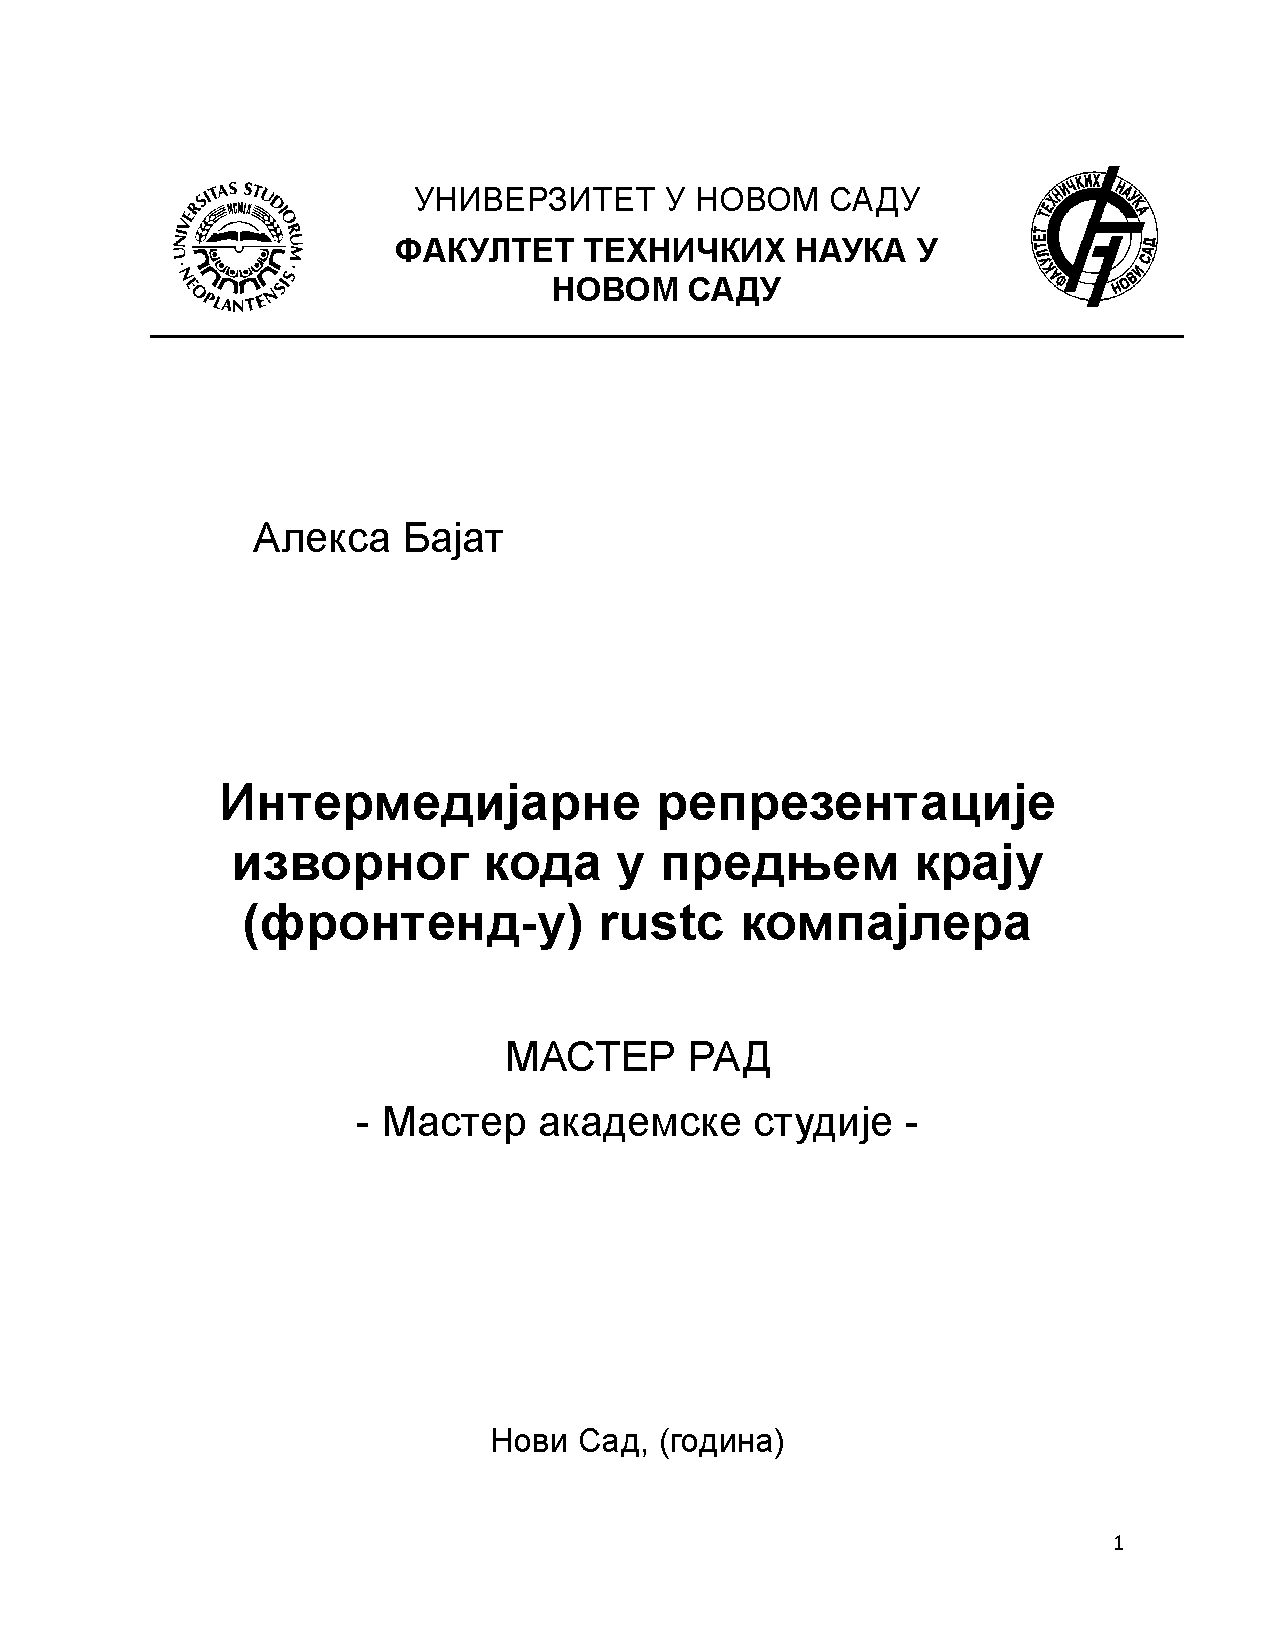
\includepdf[pages={1-6}]{MscTemplate.pdf}
\newpage
\section{Spisak skraćenica}
\newpage
\tableofcontents
\newpage

\section{Uvod}

U svetu razvoja sistema visokih performansi, operativnih sistema, drajvera i bilo kog drugog kritičnog softvera koriste se jezici niskog nivoa kao što su C i C++.
Tokom godina Microsoft je uvideo da je preko 70\% bezbednosnih slabosti nastalo pogrešnom manipulacijom i korupcijom memorije [1]. 
C nema odbrambene mehanizme od ovakvih problema (pored potencijalnih dodatnih upozorenja koja se mogu ostvariti dvostrukom upotrebom GCC i Clang kompajlera), dok C++ uprkos dodavanju konstrukta kao što su \verb|unique_ptr|, \verb|shared_ptr| i \verb|weak_ptr| interoperabilnost sa starijim standardima ili bibliotekama zahteva korišćenje sirovih pokazivača. 

Rust jezik je nastao sa ciljem da reši ovaj problem. Podrazumevana upotreba jezika je inherentno bezbedna sa aspekta memorije i paralelizma. Bezbednost se ostvaruje robustnim sistemom tipova, novog načina rukovanja memorijom i veoma striktnog \verb|rustc| kompajlera.
U C++ ekosistemu koriste se softverski obrasci kao što je \verb|Scope-bound Resource Management| da bi se standardizovala alokacija i dealkoacija memorije, ali korisnik jezika nije primoran da softvrski obrazac upotrebi. U Rust jeziku izbor ne postoji, na kraju svakog opsega vrši se automatska dealokacija memorije preko \verb|borrow checker| mehanizma (nije potreban manuelni poziv \verb|free|).
C i C++ poseduju veoma dvosmislene i neprecizne poruke kada se greška dogodi dok Rust jezik karakterišu veoma precizne poruke koje opisuju gde se desila greška i kako je potencijalno rešiti.

Prvobitna verzija Rust kompajlera je napisana u \verb|O'Caml| jeziku, dok je svaka sledeća verzija napisana u samom Rust-u.
Medjutim treba imati na umu da je Rust samo \verb|frontend| nad \verb|LLVM|-om. LLVM je kolekcija modularnih i ponovo iskoristivih tehnologija za izradu kompajlera. Rust se oslanja u potpunosti na \verb|LLVM| prilikom generisanja mašinskog koda, dok je svaki drugi deo
(\verb|frontend|) napisan potpuno ispočetka.
Veliki deo Rust jezika je izuzetno inovativan i samim tim to je razlog da se detaljno istraži kako u pozadini funkcioniše.

Reprezentacija izvornog koda jeste prikaz ili skup prikaza izvornog koda korisnika jezika koji obezbedjuju tipove, dijagnostiku,
automatsku dealokaciju memorije i ostale ergonomske i funkcionalne delovi jezika.
\newpage


\section{Verzije Rust kompajlera}

Rust kompajler u svakom trenutku poseduje tri glavne verzije skupa alata (\verb|toolchain|):

\begin{enumerate}
    \item \verb|Stable| - preporučena za svakodnevnu upotrebu. 
    \item \verb|Beta| - sa funkcionalnostima koje se usvajaju u sledećoj stabilnoj verziji (\verb|beta| postaje \verb|stable|).
    \item \verb|Nightly| - sa eksperimentalnim/nestabilnim funkcionalnostima. 
\end{enumerate}

Verzija skupa alata se može promeniti na više načina ali najjednostavniji je prikazan u izvornom kodu \ref{lst:rustup_set}.

\begin{listing}[H]
\begin{minted}{text}
    rustup toolchain install [version]
    rustup override set [version]
\end{minted}
\caption{Podešavanje verzije skupa alata}
\label{lst:rustup_set}
\end{listing}

Za prikaz dostupnih lokalnih verzija, kao i trenutna aktivna verzija u direktorijumu koristi se \verb|rustup| \ref{lst:rustup_show}.

\begin{listing}[H]
\begin{minted}{text}
    rustup show

    # IZLAZ
    installed toolchains
    --------------------
    
    stable-x86_64-unknown-linux-gnu (default)
    nightly-x86_64-unknown-linux-gnu
    
    active toolchain
    ----------------

    nightly-x86_64-unknown-linux-gnu (directory 
    override for '/home/abajat/Documents/projects/master')
    rustc 1.83.0-nightly (12b26c13f 2024-09-07)
\end{minted}
\caption{Prikaz dostupnih i trenutne verzije skupa alata}
\label{lst:rustup_show}
\end{listing}

Rust ima obećanje da će zauvek biti kompatibilan unazad uprkos konstantnom razvoju. 
\todo{Može da se proširi pričom o edicijama. \url{https://doc.rust-lang.org/edition-guide/editions/}}

\newpage

\section{Upotreba Rust kompajlera}

\verb|Rust| kompajler \verb|rustc| sa sastoji iz izuzetno velikog broja modula. 
Medjutim upotreba kompajlera je krajnje jednostavna.
Izvorni kod se upiše u tekstualni dokument i poziva rustc naredba \ref{lst:rustc}, 
nakon koje se kreira izvršni fajl pod istim imenom (pod uslovom da je kod ispravan).
\begin{listing}[H]
\begin{minted}{text}
    rustc filename.rs
\end{minted}
\caption{Pokretanje kompajlera}
\label{lst:rustc}
\end{listing}
Napredni korisnici Rust-a upotrebom promenljivih okruženja i zastavica funkcionalnosti 
(\verb|feature flag|) uvode ili menjaju osnovno ponašanje \verb|rustc| kompajlera.
Funkcionalnosti korisne za razvoj Rust kompajlera su omogućene samo u \verb|Nightly| verziji koje se
ispoljavaju preko -Z (nestabilnih) zastavica. Stabilne i nestabilne zastavice se mogu prikazati upotrebom
komandi iz isečka \ref{lst:rustc_flags}.

\begin{listing}[H]
\begin{minted}{text}
    rustc -C help # stabilne zastavice 
    rustc -Z help # nestabilne zastavice 
\end{minted}
\caption{Stabilne i nestabilne zastavice}
\label{lst:rustc_flags}
\end{listing}

Prilikom razvoja programa napisanog u \verb|Rust|-u retko se koristi direktan poziv \verb|rustc|-u već mu 
se implicitno pristupa preko menadžera paketa \verb|Cargo| \ref{lst:rustc_flags_2}. 

\begin{listing}[H]
\begin{minted}{text}
    cargo build # pokretanje kompajlera
    cargo rustc -- -C help # stabilne zastavice 
    cargo rustc -- rustc -Z help # nestabilne zastavice 
\end{minted}
\caption{Kompajliranje, stabilne i nestabilne zastavice u "Cargo" paketnom menadžeru}
\label{lst:rustc_flags_2}
\end{listing}

U Rustu, \verb|Crate| je najmanja jedinica organizacije koda. Postoje dva osnovna tipa:

\begin{enumerate}
    \item Izvršni programi - sadrže funkciju \verb|main| i mogu da se izvršavaju.
    \item Bilioteke - pružaju funkcionalnosti koje se mogu koristiti u drugim \verb|Crate|-ovima.
\end{enumerate} 

\todo{Nisam nigde prešao Query sistem, Rust ne kompajlira kroz iteracije već radi query-e. Try-mark-green algoritam je baš bitan za inkrementalnu kompilaciju.}
Rustc se odlikuje sa dva načina kompilacije: 
\begin{enumerate}
    \item Kompletna - \verb|Crate| se kompajlira od početka svaki put.
    \item Inkrementalna - prilikom kompajliranja beleži se istorija koja se koristi u svakom narednom procesu kompajliranja (dobitak u brzini na uštrb memorije).
\end{enumerate}

\section{Reprezentacije izvornog koda}

Reprezentacije izvornog koda Rust-a se dele na:

\begin{enumerate}    
    \item Tok tokena
    \item Apstraktno sintaksno stablo
    \item Posredna reprezentacija visokog nivoa
    \item Tipizirana reprezentacija visokog nivoa
    \item Reprezentacija srednjeg nivoa
    \item LLVM reprezentacija
\end{enumerate}
Sa stanovišta \verb|frontend|-a \verb|rustc| kompajlera interesantni su prvih pet nivoa. Šesti nivo generacije 
koda se naziva \verb|backend| i predstavlja \verb|FFI| (\verb|Foreign| \verb|Function| \verb|Interface|) sloj izmedju \verb|Rust|-a i \verb|C++|-a
(\verb|LLVM| je napisan u \verb|C++-u|). \todo{Da li opisati tok kompajlera i ulaziti u upoznavanje
sa svakom od ovih tačaka kroz neki pogled sa visine?}

\subsection{Tok tokena}

Uobičajno je da se lekseri programskih jezika implementiraju kao konačni automat uz pomoć alata kao što je
\verb|Flex|. Ipak, u jeziku Rust lekser je implementiran ručno. Ovo omogućava finu granularnost i visoku 
kontrolu nad procesom tokenizacije. Sa obzirom da je cilj Rust-a transparentne i korisne poruke o 
grešci, ovo je vrlo promišljena implementaciona odluka.
Kompajler poseduje naizgled dva leksera. Lekser niskog nivoa je \verb|rustc_lexer|, a lekser visokog nivoa je \verb|rustc_parse::lexer|. 
Obe implementacije su važne jer \verb|rusc_parse::lexer| koristi \verb|rustc_lexer| tokom kompajliranja.

\subsubsection{rustc\_lexer}

\verb|rustc_lexer| je lekser niskog nivoa koji poseduje sve osnovne
funkcionalnosti potrebne prilikom prikupljanja leksema.
Glavna funkcija iz ovog modula jeste \verb|tokenize| koja na osnovu celokupnog teksta 
izvornog koda dobavlja skup tokena tj. leksema \ref{lst:tokenize}.

\begin{listing}[H]
\begin{minted}{rust}
/// Creates an iterator that produces tokens from the input string.
pub fn tokenize(input: &str) -> impl Iterator<Item = Token> + '_ {
    let mut cursor = Cursor::new(input);
    std::iter::from_fn(move || {
        let token = cursor.advance_token();
        if token.kind != TokenKind::Eof { Some(token) } else { None }
    })
}
\end{minted}
\caption{Ulazna funkcija leksera}
\label{lst:tokenize}
\end{listing}

\newpage
Implementacija je bazirana na kursoru i unutar te strukture se nalazi celokupna logika leksera. 
Kursor je realizovan pomoću Rust-ovog iteratora i na osnovu njega prati trenutnu poziciju 
unutar izvornog koda. Veoma je bitna mogućnost gledanja ispred (\verb|look-ahead|) koja omogućava 
izvršavanje u jednom prolasku.
Kloniranje iteratora je jeftina operacija jer se svodi na kopiranje trenutne adresa.

\begin{listing}[H]
\begin{minted}{rust}
    /// Peeks the first symbol from the input stream without consuming it.
    pub fn first(&self) -> char {
        // `.next()` optimizes better than `.nth(0)`
        self.chars.clone().next().unwrap_or(EOF_CHAR)
    }

    /// Peeks the second symbol from the input stream without consuming it.
    pub(crate) fn second(&self) -> char {
        // `.next()` optimizes better than `.nth(1)`
        let mut iter = self.chars.clone();
        iter.next();
        iter.next().unwrap_or(EOF_CHAR)
    }

    /// Peeks the third symbol from the input stream without consuming it.
    pub fn third(&self) -> char {
        // `.next()` optimizes better than `.nth(1)`
        let mut iter = self.chars.clone();
        iter.next();
        iter.next();
        iter.next().unwrap_or(EOF_CHAR)
    }
\end{minted}
\caption{"Look-ahead" mehanizam}
\end{listing}
\verb|Token| sadrži samo informaciju o tipu token-a i njegovu dužinu ali ne i 
sam podatak.

\begin{listing}[H]
\begin{minted}{rust}
#[derive(Debug)]
pub struct Token {
    pub kind: TokenKind,
    pub len: u32,
}   
\end{minted}
\caption{Definicija "Token" strukture}
\end{listing}

\newpage
\subsubsection{rustc\_parse::lexer}

Lekser višeg nivoa \verb|rustc_parse::lexer| koristi \verb|rustc_lexer| prilikom izvršavanja sopstvenih
operacija. Bitna razlika je to što se sadržaj token analizira i postavlja u kontekst.
Lekser višeg nivoa koristi kursor svog prethodnika za dobavljanje leksema kroz strukturu \verb|StringReader|. 

\begin{listing}[H]
\begin{minted}{rust}
    struct StringReader<'psess, 'src> {
        psess: &'psess ParseSess,
        start_pos: BytePos,
        pos: BytePos,
        src: &'src str,
        cursor: Cursor<'src>,
        override_span: Option<Span>,
        nbsp_is_whitespace: bool,
        last_lifetime: Option<Span>,
    }
\end{minted}
\caption{Definicija "StringReader" strukture}
\end{listing}
\verb|StringReader| prati trenutnu poziciju unutar izvornog koda, a kursor 
dobavlja token koji ima odredjenu dužinu. Sadržaj tokena je niz karaktera sa početkom u \verb|pos|,
dužine od \verb|token.len|. 

Prolaskom kroz izvorni kod izvršavaju se sledeće akcije:
\begin{enumerate}
    \item Interniranje 
    \item Tokeni iz \verb|rustc_lexer| se mapiraju na tokene iz \verb|rustc_ast|
    \item Rezulucija zagrada svih tipova.
    \item Problemi i preporuke generišu dijagnostiku 
\end{enumerate}

Interniranje je proces u kome se stringovi pretvaraju internirane simbole. Na ovaj način
se čuva samo jedna nepromenljiva kopija sadržaja tokena. Tabela simbola je struktura podataka
koja čuva i održava O(1) pristup bilo kom simbolu.  Tabela simbola je implementirana pomoću \verb|IndexSet|
strukture. Ne internira se svaki token, već samo tokeni koji imaju varijabilnu dužinu.
\todo{Interniranje u pozadini koristi SpanData strukturu, u zavisnosti od specifičnih okolnosti
može koristiti manje ili veće Span-ove. Bitno je, ali nisam siguran da li zalaziti toliko u samu implementaciju.}

Mapiranje tokena iz leksera u tip tokena iz apstraktnog sintaksnog stabla je trivialno.
Za proste tipove vrši se jedan na jedan konverzija.

\begin{listing}[H]
\begin{minted}{rust}
    rustc_lexer::TokenKind::Semi => token::Semi,
    rustc_lexer::TokenKind::Comma => token::Comma,
    rustc_lexer::TokenKind::Dot => token::Dot,
\end{minted}
\caption{Prevodjenje tokena iz leksera u AST tokene}
\end{listing}
Za tipove koji imaju sadržaj u vidu nizova karaktera, sadržaj se internira i prenosi 
u novi token putem simbola \ref{lst:intern}. Derivati apstraktnog sintaksnog stabla se često koriste prilikom kompajliranja i zbog toga 
stablo mora biti memorijski optimizovano.

\begin{listing}[H]
\begin{minted}{rust}
    let ident = Symbol::intern(lifetime_name);
    token::Lifetime(ident, IdentIsRaw::No)
\end{minted}
\caption{Interniranje literala}
\label{lst:intern}
\end{listing}
Tok tokena je skup stabala tokena od kojih je svako stablo sačinjeno od skupa tokena.  
Rezolucija zagrada je proces unutar kog se validira da li je svaka zagrada pravilno zatvorena.
Rezolucija zagrada se dešava u samom vrhu procesa \verb|rustc_parser::lexer|-a 
za vreme kreiranja toka tokena. U kontekstu kompajlera zagrade se nazivaju delimiteri. 
Svaki otvoreni tip delimitera mora biti zatvoren delimiterom istog tipa koji je zatvoren.
Na primer, vitičasta zagrada je tip delimitera koja može biti otvoren (\{) ili zatvoren (\}) tj.
svaka otvorena vitičasta zagrada mora biti zatvorena zatvorenom vitičastom zagradom.

\begin{listing}[H]
\begin{minted}{rust}
fn lex_token_trees(
    &mut self,
    is_delimited: bool,
) -> (Spacing, TokenStream, Result<(), Vec<PErr<'psess>>>) {
    // Move past the opening delimiter.
    let (_, open_spacing) = self.bump(false);
    let mut buf = Vec::new();
    loop {
        match self.token.kind {
            token::OpenDelim(delim) => buf.push(match self
            .lex_token_tree_open_delim(delim) {
                Ok(val) => val,
                Err(errs) => return (open_spacing, 
                TokenStream::new(buf), Err(errs)),
            }),
            token::CloseDelim(delim) => {
                return (
                    open_spacing,
                    TokenStream::new(buf),
                    if is_delimited { 
                        Ok(()) 
                    } else { Err(vec![self.close_delim_err(delim)]) },
                );
            }
            token::Eof => {
                return (
                    open_spacing,
                    TokenStream::new(buf),
                    if is_delimited { Err(vec![self.eof_err()]) } 
                    else { Ok(()) },
                );
            }
            _ => {
                // Get the next normal token.
                let (this_tok, this_spacing) = self.bump(true);
                buf.push(TokenTree::Token(this_tok, this_spacing));
    } } } }
\end{minted}
\caption{Generisanje stabla tokena}
\end{listing}

\newpage

Primećuje se da u slučaju da kada delimiter ne postoji, dodavanje tokena u tok tokena 
je sekvencijalno i ne zahteva nikakvu kompleksnu logiku. Promenljiva \verb|is_delimited|
označava da li trenutna sekvenca tokena pripada nekom paru delimitera. U slučaju da 
se naidje na zatvoren tip delimitera bez da je prethodno postojao otvoren, vraća se greška
u vidu dijagnostike. U sličnom kontekstu, nailazak na token kraj-a fajla bez da je svaka 
zagrada zatvorena je greška. 
Nailaskom na \verb|token::Eof| ili \verb|token::CloseDelim| se završava prikupljanje toka tokena.
Ovo su veoma korisni granični slučajevi koji omogućavaju rekurziju. 

Obrada otvorenog tipa delimitera u pozadini poziva funkciju \verb|lex_token_trees| koji obradjuje
stablo tokena (deo toka tokena) izmedju novog para zagrada.
\begin{listing}[H]
\begin{minted}{rust}
    fn lex_token_tree_open_delim(
        &mut self,
        open_delim: Delimiter,
    ) -> Result<TokenTree, Vec<PErr<'psess>>> {
        // The span for beginning of the delimited section.
        let pre_span = self.token.span;

        self.diag_info.open_braces.push((open_delim, self.token.span));

        // Lex the token trees within the delimiters.
        // We stop at any delimiter so we can try to recover if the user
        // uses an incorrect delimiter.
        let (open_spacing, tts, res) = self
                            .lex_token_trees(/* is_delimited */ true);
        if let Err(errs) = res {
            return Err(self.unclosed_delim_err(tts, errs));
        }

        // Expand to cover the entire delimited token tree.
        let delim_span = DelimSpan::from_pair(pre_span, self.token.span);
        let sm = self.string_reader.psess.source_map();

        let close_spacing = match self.token.kind {
        .
        .
        .
\end{minted}
\caption{Parsiranje stabla tokena}
\end{listing}

Neobradjene zagrade se čuvaju u strukturi \verb|TokenTreeDiagInfo| u polju \verb|open_braces|.
Utvrdjeno je da će po uspešnom završetku izvršavanja funkcije \verb|lex_token_trees| 
trenutni token biti pozicioniran na zatvoreni tip delimiter-a. To omogućava validaciju 
pravilnog završetka zagrada.

\newpage
\subsection{Apstraktno Sintaksno Stablo}

Parser jezika Rust uz pomoć toka tokena iz leksera generiše apstraktno sintaksno stablo (AST). 
Prilikom poziva parsiranja, jedini fajl koji se odmah procesira jeste glavni \verb|main| fajl, potpuno stablo
nastaje putem ekspanzije i rezolucije imena.
Algoritam \verb|recursive-descent| se koristi tokom procesa parsiranja. Ovo je jedna od najjednostavnijih
tehnika parsiranja koja se koristi u praksi. Ovakvi parseri se takodje nazivaju \verb|top-down| parseri 
jer konstruišu stablo od gore ka dole \cite{parsing}. 

Parser koristi prethodno pomenuti tok tokena da bi kreirao kursor nad stablom tokena \verb|TokenTreeCursor|.
\verb|TokenStream| poseduje implementaciju \verb|into_tree| koji transformiše tip dobijen iz leksera
u tip pogodan parseru.

\begin{listing}[H]
\begin{minted}{rust}
pub fn into_trees(self) -> TokenTreeCursor {
    TokenTreeCursor::new(self)
}

impl TokenTreeCursor {
    fn new(stream: TokenStream) -> Self {
        TokenTreeCursor { stream, index: 0 }
    }
    ...
}
\end{minted}
\caption{Konverzija iz "TokenStream" u "TokenTreeCursor"}
\end{listing}
Jednostavnije je iterirati kroz stabla tokena sekvencijalno u odnosu na strukturu koja liči na kanape.

Za razliku od leksera, parser poseduje konstrukte koji su dosta složeniji od jednog tokena, kao što su 
strukture, enumeracije i slično (reč-rečenica poredjenje). Izvorni čvor \verb|AST|-a je \verb|Crate|.

\begin{listing}[H]
\begin{minted}{rust}
#[derive(Clone, Encodable, Decodable, Debug)]
pub struct Crate {
    pub attrs: AttrVec,
    pub items: ThinVec<P<Item>>,
    pub spans: ModSpans,
    pub id: NodeId,
    pub is_placeholder: bool,
}
\end{minted}
\caption{Definicija "Crate" strukture}
\end{listing}

\newpage

Najbitnija polja su atributi (\verb|attrs|) i stavke (\verb|items|). Atributi mogu biti spoljašnji ili unutrašnji.
Koriste se da bi korisnik pružio dodatne instrukcije kompajleru. 
Dodatne instrukcije mogu biti trivijalne poput dozvoljavanja
nekorišćenog koda, ali mogu biti i kompleksnije u vidu implementacije osobina 
(\verb|trait|). Osobina je funkcionalnost veoma slična interfejsu u drugim jezicima. 


\begin{listing}[H]
\begin{minted}{rust}
// Spoljašnji atribut se primenjuje na tip koji sledi 
// nakon atributa koji pri tome nije atribut.
#[allow(dead_code)] 
fn main() {
    // Unutrašnji atribut.
    // Primenjuje se na vlasnika lokalnog opsega. 
    #![allow(unused_variables)]
    let x = 10;  
}
\end{minted}
\caption{Spoljašnji i unutrašnji atributi}
\end{listing}


Stavke su grupacije tokena iz leksera koje tako grupisane imaju semantiku. Iz perspektive koda 
veoma se malo razlikuje od samog \verb|Crate|-a. Svaka stavka poseduje identifikator \verb|NodeId| 
koji predstavlja sekvencijalni broj stavke unutar \verb|Crate|-a. Ovo znači da ukoliko se usred stabla 
obriše ili izgeneriše nova stavka, svaki čvor nakon tog dela stabla mora ponovo da izgeneriše svoj redni broj.
Samim time apstraktno sintaksno stablo nije korisno prilikom inkrementalne kompilacije jer su identifikatori
volotilni. Svaka stavka takodje sadrži \verb|Span|. Ovo je tip koji odredjuje početnu i krajnju poziciju 
stavke unutar izvornog koda. U odnosu na vrednost tipa \verb|kind|, stavke mogu ili ne mogu da poseduju atribute. 

\begin{listing}[H]
\begin{minted}{rust}
#[derive(Clone, Encodable, Decodable, Debug)]
pub struct Item<K = ItemKind> {
    pub attrs: AttrVec,
    pub id: NodeId,
    pub span: Span,
    pub vis: Visibility,
    pub ident: Ident,
    pub kind: K,
    pub tokens: Option<LazyAttrTokenStream>,
}
\end{minted}
\caption{Definicija "Item" strukture}
\end{listing}

\begin{listing}[H]
\begin{minted}{rust}
pub fn parse_crate_mod(&mut self) -> PResult<'a, ast::Crate> {
    let (attrs, items, spans) = self.parse_mod(&token::Eof)?;
    Ok(ast::Crate { attrs, items, spans, 
       id: DUMMY_NODE_ID, is_placeholder: false })
}
\end{minted}
\caption{Ulazna funkcija parsera}
\end{listing}


Rezolucija imena je jedan od delova formiranja apstraktnog sintaksnog stabla.
U programima se referenciraju funkcije, varijable i tipovi na osnovu imena. Ova imena nisu uvek jedinstvena.

\begin{listing}[H]
\begin{minted}{rust}
type a = u32;
let a: a = 1;
let b: a = 5; 
\end{minted}
\caption{Rezolucija imena}
\label{lst:resolution}
\end{listing}

Kako znamo, u izvornom kodu \ref{lst:resolution}, da li je u liniji 3 "a" tip ili vrednost 1?
Ovakvi konflikti se rešavaju prilikom rezolucije imena. U datom slučaju imena tipova i promenljivih se nalaze 
u različitim imenskim prostorima (\verb|namespaces|) i zbog toga mogu da koegzistiraju.
Rezolucija imena se izvodi iz dva faze. Prva faza se dešava za vreme ekspanzije (više o tome u daljem tekstu) 
gde se obradjuju samo \verb|import|-i. Druga faza se dešava nakon ekspanzije gde se obradjuje celokupno 
sintaksno stablo počevši od vrha pa na dole. 

Imena su validna u različitim delovima izvornog koda. Da bi se 
vreme života (\verb|scope|) nekog imena proverilo uvodi se koncept rebara (\verb|rib|). Svaki put kada se 
set vidljivih imena potencijalno menja novo rebro se gura na stek. Primeri situacija u kojima se dodaje 
novo rebro:
\begin{enumerate}
    \item Očigledna mesta kao što su vitičaste zagrade, funkcije, moduli.
    \item Prilikom poziva \verb|let| jer se ime može redefinisati (\verb|shadowing|).
    \item Početak proširenja makroa. 
\end{enumerate}
Potraga za imenom se izvodi od najdubljeg rebra (vrh steka) ka najplićem. 
Redosled je veoma bitan zato što se ovakvom pretragom izbegava greška 
ukoliko je neko ime redefinisano.

\begin{listing}[H]
\begin{minted}{rust}
let a: u32 = 1;
let a: i32 = -1;
\end{minted}
\caption{"Shadowing"}
\label{lst:shadowing}
\end{listing}
\newpage

Jezici kao što je C pored kompajlera sadrže pre-procesor koji prikuplja izvorni kod. 
Prilikom prikupljanja izvornog koda skraćenice (makroi) se proširuju na izraze programskog jezika. 
Rust se odlikuje veoma moćnim makroima ali ne poseduje pre-procesor. Transformacija skraćenica se vrši 
putem ekspanzije.  Ekspanzija je proces tokom kog se dopunjuje apstraktno sintaksno stablo
proširivnajem makroa i umetanjem modula (\verb|inlining|). Prilikom parsiranja umesto 
modula i makroa se postavljaju AST fragmenti. Ovi fragmenti su početne tačke algoritma ekspanzije.
Kreira se red čekanja neproširenih makroa. Jedan po jedan se uzimaju iz reda čekanja, vriši se rezolucija imena,
proširuju se i integrišu nazad u stablo. U slučaju da se nema napretka (loše napisan kod), vraća se greška.

Pre nego što počne prelazak u sledeći posredni oblik AST stablo se validira. 
Tokom prolaska se proverava da li je stablo sintaktički validno, bez ikakvih kompleksnih analiza,
rezolucije imena ili provera tipova. Ovo nije moguće učiniti prilikom parsiranja jer makro atributi 
omogućavaju odredjene delove netačne sintakse kao što je funkcija bez tela van definicije osobine (\verb|trait|) \ref{lst:validate}.

\begin{listing}[H]
\begin{minted}{rust}
#[attribute]
mod foo {
    fn missing_body();
}
\end{minted}
\caption{"Netačna sintaksa pre ekspanzije"}
\label{lst:validate}
\end{listing}
\todo{Mogu da napišem makro koji bi proširio telo funkcije, da li da dodam?}

Apstraktno sintaksno stablo pre i posle ekspanzije nekog \verb|Crate|-a se može analizirati pomoću 
nestabilnih \verb|-Z| zastavica \ref{lst:rustc_ast}.

\todo{Sam prikaz AST-a nije naročito interesantan, a čak i za najjednostavnije programe a + b ume da bude 
pozamašne dužine}

\begin{listing}[H]
\begin{minted}{bash}
cargo rustc -- -Z unpretty=ast
cargo rustc -- -Z unpretty=ast,expanded
\end{minted}
\caption{"Prikaz apstraktnog sintaksnog stabla"}
\label{lst:rustc_ast}
\end{listing}

\newpage
\subsection{Posredna Reprezentacija Visokog Nivoa - HIR (High-Level Intermediate Representation)}

Posredna reprezentacija visokog nivoa je primarna posredna reprezentacija koja se koristi 
u većinskom delu \verb|rustc| kompajlera. HIR je posledica snižavanja (\verb|lowering|). 
Tokom procesa snižavanja, neke forme izražavanja bivaju pojednostavljene (\verb|desugared|):
\begin{enumerate}
    \item Zagrade se uklanjaju jer struktura stabla eksplicitno odredjuje redosled operacija.
    \item for petlje su konvertovane u while(let) petlje \ref{lst:hir_iter}.
    \item if let se konvertuje u match.
    \item impl u parametrima funkcije se konvertuje u generičke argumente.
\end{enumerate}

\begin{listing}[H]
\begin{minted}{rust}
// Pre
for elem in vec {
    process(elem);
}

// Posle
let mut iterator = vec.into_iter();
while let Some(elem) = iterator.next() {
    process(elem);
}
\end{minted}
\caption{"for" petlja pre i posle pojednostavljenja}
\label{lst:hir_iter}
\end{listing}

HIR prikazuje samo trenutno stanje \verb|Crate|-a.
Samim time sadrži samo funkcije drugih modula koje su implicitno ili eskplicitno korišćene 
od strane glavnog modula, sve ostalo će biti ignorisano.

Glavni čvor HIR-a se isto kao i kod AST-a naziva \verb|Crate| ali sadrži drugačije podatke,
veliki broj mapa koje služe da omoguće lakši pristup sadržaju.

HIR poseduje proširen spektar identifikatora:
\begin{enumerate}
    \item DefId - referencira definiciju unutar bilo kog \verb|Crate|-a.
    \item LocalDefId - referencira definiciju unutar trenutno kompajliranog \verb|Crate|-a.
    \item HirId - referencira bilo koji čvor u HIR-u.
\end{enumerate}

Većinu vremena HIR-u se pristupa pomoću HIR mape. HIR mapa sadrži brojne metode 
koje na osnovu različitih tipova identifikatora dobavljaju podatke.
\todo{Nisam zadovoljan ovim delom, potrebno je ako ništa objasniti zašto su ovi identifikatori korisni
u vidu inkrementalne kompilacije}

\newpage
\subsection{Tipizirana Posredna Reprezentacija Visokog Nivoa - THIR (Typed High-Level Intermediate Representation)}

Tipizirani HIR je posredna reprezentacija izvornog koda koja se generiše tokom provere tipova, jer je potrebno
da su tipovi unutar celog stabla popunjeni. THIR sadrži samo tela (obično tela funkcija) tj. izvršni kod.
Posledica ovoga jeste nedostatak reprezentacija struktura i osobina. 
Rust ima odliku da ukoliko se koristi neki vid provere šablona (\verb|pattern matching|) svaki tip unutar 
šablona mora biti pokriven \ref{lst:pattern_matching}. Proveru da li je svaki tip obradjen izvršava THIR.

\begin{listing}[H]
\begin{minted}{rust}
pub enum IpAddrKind {
    V4,
    V6,
}

fn main() {
    let x = IpAddrKind::V4;
    match x {
        IpAddrKind::V4 => println!("Ovo je IPv4 adresa."), 
        // Pokriven IpAddrKind::V4
        IpAddrKind::V6 => println!("Ovo je IPv6 adresa.") 
        // Pokriven IpAddrKind::V6
        // Da je postojao IpAddrKind::V7 Rust bi zahtevao 
        // da i ta varijanta bude obradjena.
    }
}
\end{minted}
\caption{Provera šablona}
\label{lst:pattern_matching}
\end{listing}

Za razliku od HIR-a koji je perzistiran tokom celokupnog izvršavanja kompajlera, THIR se odbacuje momenta
kada više nema upotrebnu vrednost. Pored toga što su svi tipovi čvorova prisutni, THIR se odlukuje dodatnim 
pojednostavljivanjem koda:
\begin{enumerate}
    \item Automatska referenciranja i dereferenciranja su eksplicitna.
    \item Pozivi metoda i opterećeni operatori su konvertovani u obične pozive funkcija. 
    \item Obim životnog veka je eksplicitan.
\end{enumerate}
% Izrazi, iskazi i \verb|match| ruke se čuvaju zasebno. 

Pojednostavljenje čini THIR podobnim za proveru nebezbednog koda jer fundamentalno poseduje manje opcija, 
nebezbedni pozivi metoda i nebezbedni pozivi funkcija imaju identičnu reprezentaciju. Ova provera 
iskazuje grešku ako je nebezbedna operacija korišćena van \verb|unsafe| opsega.

\todo{THIR je kratak sam po sebi ali moguće je detaljnije obraditi pattern matching}

\newpage
\subsection{Posredna Reprezentacija Srednjeg Nivoa - MIR (Mid-Level Intermediate Representation)}

Prvobitno koncept \verb|MIR|-a nije postojao. HIR se transformisao u LLVM reprezentaciju gde 
vršila optimizacija. Glavni povod za uvod reprezentacije srednjeg nivoa 
jeste inkrementalna kompilacija i MIR je struktuiran tako da ga je lako sačuvati i učitati, iako su se delovi
koda promenili tokom vremena.

U HIR-u optimizacija \verb|for| petlje je svedena na \verb|while(let)| u MIR-u se prevodi na \verb|loop match| 
primitivu \ref{lst:mir_for_1}.  Pozivi metoda su prevedeni u pozive funkcija još u THIR-u.

\begin{listing}[H]
\begin{minted}{rust}
let mut iterator = IntoIterator::into_iter(vec);
loop {
    match Iterator::next(&mut iterator){
        Some(elem) => process(elem),
        None => break,
    }
}
\end{minted}
\caption{"while let" posle pojednostavljenja}
\label{lst:mir_for_1}
\end{listing}

Reprezentacija srednjeg nivoa dozvoljava za još jedan vid optimizacije na nivou frontenda pojednostavljivanjem
sintakse na primitive koje nisu dostupne u regularnom jeziku.

\begin{listing}[H]
\begin{minted}{rust}
let mut iterator = IntoIterator::into_iter(vec);

loop:
    match Iterator::next(&mut iterator) {
        Some(elem) => { process(elem); goto loop; }
        None => { goto break; }
    }

break:
\end{minted}
\caption{"while let" posle pojednostavljenja}
\label{lst:mir_for_2}
\end{listing}

Izraz \verb|goto| je u inženjerskoj zajednici gledan sa visine jer kontrola toka nakon odredjene kompleksnosti
postaje nerazumljiva. Rust iz istog razloga ne dozvoljava upotrebu ove ključne reči, ali u MIR-u svodi 
petlju na najjednostavniji oblik \ref{lst:mir_for_2}.

\newpage
U isečku koda \ref{lst:mir_for_2}, jedina kompleksnija sintaktička celina je \verb|match|. U samom jeziku 
grupisanje provere i pristup podatku je smisleno ali u MIR-u se odvaja na dve celine \ref{lst:mir_for_3}.

\begin{listing}[H]
\begin{minted}{rust}
loop:
    let tmp = Iterator::next(&mut iterator);
    
    switch tmp {
        Some => {
            let elem = (tmp as Some).0;
            process(elem);
            goto loop;
        }
        None => {
            goto break;
        }
    }
    
break:
    ....
\end{minted}
\caption{"while let" posle pojednostavljenja}
\label{lst:mir_for_3}
\end{listing}

Naime ovako sveden kod nikada nije tekstualnom obliku. MIR je graf kontrole toka koji se može predstaviti
uz pomoć \verb|graphviz|-a \ref{lst:mir_print}. Filter mora biti zadatat prilikom poziva ove komande. 
Za prikaz celokupnog izlaza koristi se \verb|all| filter, dok ako je neka pojedinačna funkcija od interesovanja
njeno ime (mnogo češće slučaj).

\begin{listing}[H]
\begin{minted}{bash}
cargo rustc -- -Z dump-mir=[filter] -Z dump-mir-graphviz
\end{minted}
\caption{Ispis i prikaz MIR-a}
\label{lst:mir_print}
\end{listing}

\todo{MIR je opsežan, ne izgleda kao u primerima (umereni nivo obfuskacije). Ovde ima još značajno puno sadržaja koji nije opisan.}
\newpage
\section{Zaključak}

\newpage
\section{Literatura}

\begin{thebibliography}
    \raggedright
\bibitem{msrc} 
    MSRC, “A proactive approach to more secure code | MSRC Blog | 
    Microsoft Security Response Center,” Microsoft.com, Jul. 16, 2019. 
    \url{https://msrc.microsoft.com/blog/2019/07/a-proactive-approach-to-more-secure-code/} 
    (pristupljeno Sep. 08, 2024).

    \bibitem{parsing} 
    “Parsing” Rochester.edu, 2024.
    \url{https://www.cs.rochester.edu/u/nelson/courses/csc_173/grammars/parsing.html#:~:text=Recursive%2Ddescent%20parsing%20is%20one,non%2Dterminal%20with%20a%20procedure} 
    (pristupljeno Sep. 21, 2024).

    \bibitem{dragonbook} 
    A. V. Aho, M. S. Lam, R. Sethi, and J. D. Ullman, \emph{Compilers: Principles, Techniques, and Tools}, 2nd ed. Boston, MA, USA: Addison-Wesley, 2006.

    \bibitem{rust-guide} 
    “Getting Started - Rust Compiler Development Guide,” Rust-lang.org, 2024. 
    \url{https://rustc-dev-guide.rust-lang.org/getting-started.html} (accessed Sep. 28, 2024).

    \bibitem{rust-reference}
    “Introduction - The Rust Reference,” Rust-lang.org, 2015. 
    \url{https://doc.rust-lang.org/reference/introduction.html} (accessed Sep. 29, 2024).
    
    \bibitem{rustonomicon}
    “Meet Safe and Unsafe - The Rustonomicon,” Rust-lang.org, 2024. 
    \url{https://doc.rust-lang.org/nomicon/meet-safe-and-unsafe.html} (accessed Sep. 29, 2024).
\end{thebibliography}

\newpage
\section{Podaci o kandidatu}


Kandidat Aleksa Bajat rođen je 2001. godine u Novom Sadu. Završio je prirodno-matematički smer na engleskom jeziku 
u gimnaziji "Jovan Jovanović Zmaj" 2019. godine. Tokom sve četiri godine gimnazije uspešno je pohadjao 
"Centar za mlade talente" kompanije Schneider Electric.  Godine 2019. upisao je Fakultet 
Tehničkih Nauka u Novom Sadu, gde je ispunio sve obaveze i položio sve ispite predviđene 
studijskim programom sa prosečnom ocenom 9.03.

\end{document}
